\documentclass[12pt]{article}
\usepackage[paper=letterpaper,margin=2cm]{geometry}
\usepackage{amsmath}
\usepackage{amssymb}
\usepackage{amsfonts}
\usepackage{newtxtext, newtxmath}
\usepackage{enumitem}
\usepackage{titling}
\usepackage[colorlinks=true]{hyperref}
\usepackage{graphicx}
\usepackage{csvsimple}
\usepackage{luacode}
\documentclass{article}

\usepackage{algorithm}
\usepackage{algpseudocode}
\setlength{\droptitle}{-6em}

% Enter the specific assignment number and topic of that assignment below, and replace "Your Name" with your actual name.

\title{\textbf{COMP0078 Assignment 2}}
\author{Student Numbers: 21168615 \& 19004608 \\ }
\date{Dec 14, 2022}

\begin{document}
    \maketitle
\section{PART I}
\subsection{Kernel Perceptron}
\subsubsection{Experimental Results}

\begin{itemize}
    \item[1.] To generalise the kernel perceptron to $K$ classes:
    \begin{algorithm}
    \caption{An training algorithm for multi-class kernel perceptron}\label{alg:cap}
    \begin{algorithmic}
    \For{$k\in\{1, 2, ..., K\}}$ \Comment Initialise weights for first training example
        \State $w^{1, 1}_k \gets 0$
    \EndFor

    \For{$i\in\{1, 2, ..., M\}$}: \Comment Number of Epochs
        \For{$j\in\{2, ..., N\}}$ \Comment Number of training points (skipping the first point)
            \For{$k\in\{1, 2, ..., K\}}$ \Comment Number of classes
                \State $\hat{y}_k^{i, j} \gets  \sum_{i'=1}^{i-1} \sum_{j'=1}^{j-1} ( w^{i', j'}_k \cdot  k(\textbf{x}_{j'}, \textbf{x}_j)} )$ \Comment{Prediction for class $k$ with kernel $k(\cdot, \cdot)$}
                \If{$sign(\hat{y}_k^{i, j}) \neq sign(y_k^{i, j})$} \Comment Compare predicted $\hat{y}_k^{i, j}$ and actual $y_k^{i, j})$
                    \State $w^{i, j}_{k} \gets y_k^{i, j}$
                \Else
                    \State $w^{i, j}_{k} \gets 0$
                \EndIf
            \EndFor
        \EndFor
    \EndFor
    \end{algorithmic}
    \end{algorithm}

    The number of epochs was determined by training on the mini training data set until the performance of the mini testing data set no longer changed.
    This was considered a reasonable number of epochs to use to train the actual data set.

    For prediction, the $k$ with the maximum value of $\hat{y}_k$ (the argmax of $\hat{y}$) is considered the label prediction by the model.
    \newpage

    Basic Results:

    \begin{figure}[h]
    \centering
    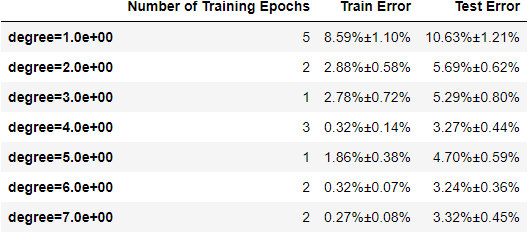
\includegraphics[scale=0.5]{outputs/part1/q1.png}
    \caption{20 Runs with a Polynomial Kernel}
    \label{fig:1}
    \end{figure}

    \item[2.] Cross Validation Results:

    \begin{figure}[h]
    \centering
    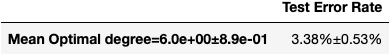
\includegraphics[scale=0.5]{outputs/part1/q2.png}
    \caption{5-fold Cross-Validation for 20 Runs with a Polynomial Kernel}
    \label{fig:2}
    \end{figure}
\newpage

    \item[3.] Confusion Matrix:

    \begin{figure}[h]
    \centering
    \begin{minipage}{.5\textwidth}
      \centering
      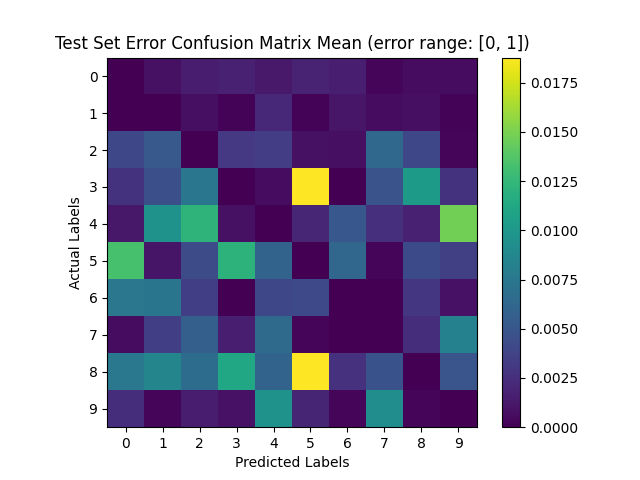
\includegraphics[width=.8\linewidth]{outputs/part1/q3_confusion-imshow_mean.png}
      \caption{Polynomial Kernel Mean}
      \label{fig:3}
    \end{minipage}%
    \begin{minipage}{.5\textwidth}
      \centering
      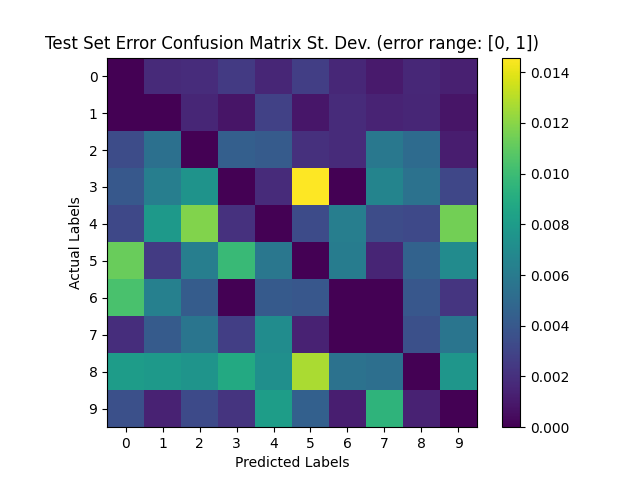
\includegraphics[width=.8\linewidth]{outputs/part1/q3_confusion-imshow_stdev.png}
      \caption{Polynomial Kernel St. Dev.}
      \label{fig:4}
    \end{minipage}
    \end{figure}

    \begin{figure}[h]
    \centering
    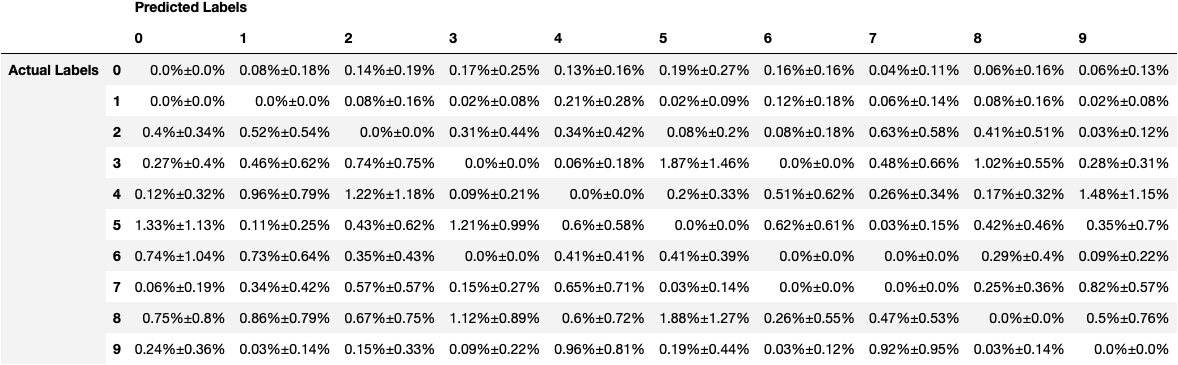
\includegraphics[scale=0.5]{outputs/part1/q3_confusion.png}
    \caption{Polynomial Kernel Confusion Matrix Error Rate Table}
    \label{fig:5}
    \end{figure}


    \item[4.] The images with the most errors made by the 20 models trained in part 2 were considered the hardest to predict and visualised.
    It is not surprising that these are hard to predict.
    We can see that in all five cases, the images do not look like their labels, in fact, they mostly look like vertical or horizontal bars.
    Thus it would be unreasonable to expect a model to predict them correctly.

    \begin{figure}[h]
    \centering
    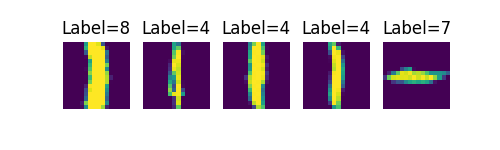
\includegraphics[scale=0.7]{outputs/part1/q4.png}
    \caption{Images with the Most Errors from the Trained Models}
    \label{fig:6}
    \end{figure}

    \newpage

    \item[5.] To select a good range of values for the kernel width sigma for the Gaussian kernel, the mini training and testing sets was used to quickly gauge the test error for different hyper-parameters.
    The hyper-parameter values above and below the best performing hyper-parameter (with respect to test set error) was chosen as the hyper-parameter range to define $S$, the set of values for cross-validation for repeating parts 1 and 2 with the Gaussian Kernel.
    \begin{figure}[h]
    \centering
    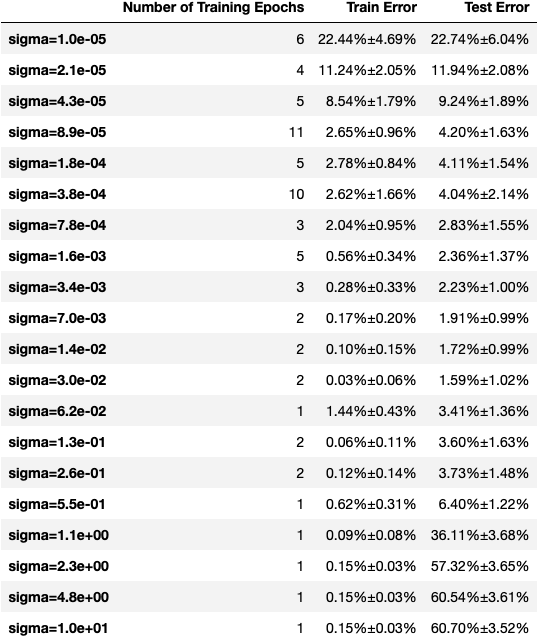
\includegraphics[scale=0.5]{outputs/part1/q5_1-mini.png}
    \caption{Performance for mini data set (to narrow down a hyper-parameter range)}
    \label{fig:7}
    \end{figure}
    \newpage

    Basic Results:

    \begin{figure}[h]
    \centering
    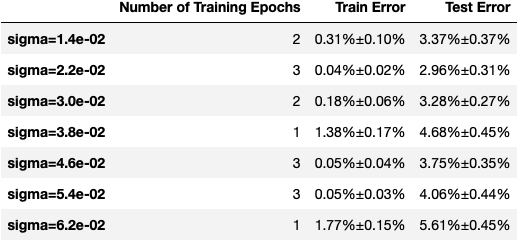
\includegraphics[scale=0.5]{outputs/part1/q5_1.png}
    \caption{20 Runs with a Gaussian Kernel}
    \label{fig:8}
    \end{figure}


    Cross Validation Results:

    \begin{figure}[h]
    \centering
    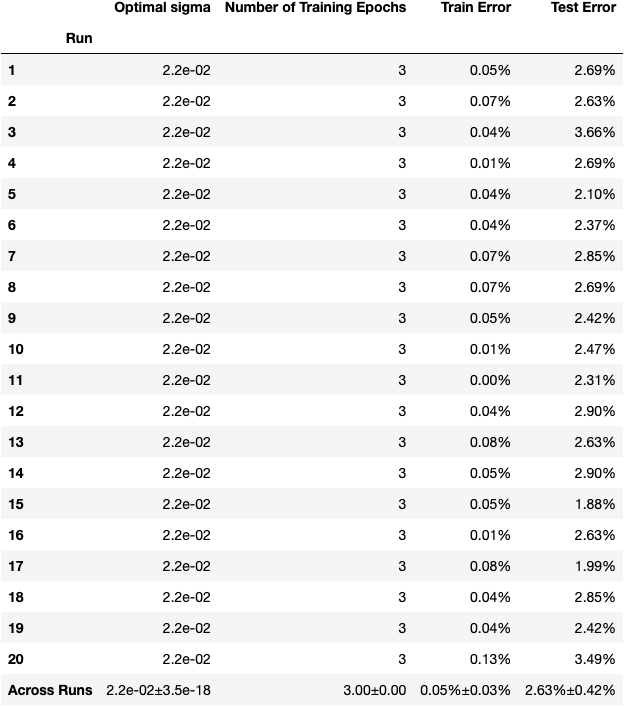
\includegraphics[scale=0.5]{outputs/part1/q5_2.png}
    \caption{5-fold Cross-Validation for 20 Runs with a Gaussian Kernel}
    \label{fig:9}
    \end{figure}

\newpage
    \item[6.] An alternative method to generalise the kernel perceptron to $k$-classes:

    \begin{algorithm}
    \caption{Another training algorithm for multi-class kernel perceptron}\label{alg:cap}
    \begin{algorithmic}
    \For{$k\in\{1, 2, ..., K\}}$ \Comment Initialise weights for first training example
        \State $w^{1, 1}_k \gets 0$
    \EndFor

    \For{$i\in\{1, 2, ..., M\}$}: \Comment Number of Epochs
        \For{$j\in\{2, ..., N\}}$ \Comment Number of training points
            \For{$k\in\{1, 2, ..., K\}}$ \Comment Number of classes
                \State $\hat{y}_k^{i, j} \gets  \sum_{i'=1}^{i-1} \sum_{j'=1}^{j-1} ( w^{i', j}_k \cdot  k(\textbf{x}_{j'}, \textbf{x}_j)} )$ \Comment{Prediction for class $k$ with kernel $k(\cdot, \cdot)$}
            \EndFor
            \State $\hat{c} \gets argmax_k \hat{y}_k^{i, j}$ \Comment Predicted label
            \State $c \gets argmax_k y_k^{i, j}$ \Comment Actual label
            \If{$\hat{c} \neq c$} \Comment Compare predicted and actual label
                \State $w^{i, j}_{c} \gets y_{c}^{i, j}$ \Comment Non-zero weights only for actual and predicted label
                \State $w^{i, j}_{\hat{c}} \gets y_{\hat{c}}^{i, j}$
                \State $w^{i, j}_{k} \gets 0 \forall k\in\{1, 2, ..., K\}, k \neq c, k\neq \hat{c}$
            \Else \Comment All zero weights if actual and predicted labels match
                \State $w^{i, j}_{k} \gets 0 \forall k\in\{1, 2, ..., K\}$
                \EndIf
        \EndFor
    \EndFor
    \end{algorithmic}
    \end{algorithm}
\newpage

    Basic Results:

    \begin{figure}[h]
    \centering
    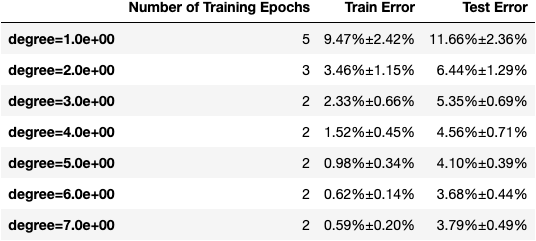
\includegraphics[scale=0.5]{outputs/part1/q6.png}
    \caption{20 Runs with a Polynomial Kernel (Alternative Training Method)}
    \label{fig:10}
    \end{figure}
    Cross Validation Results:

    \begin{figure}[h]
    \centering
    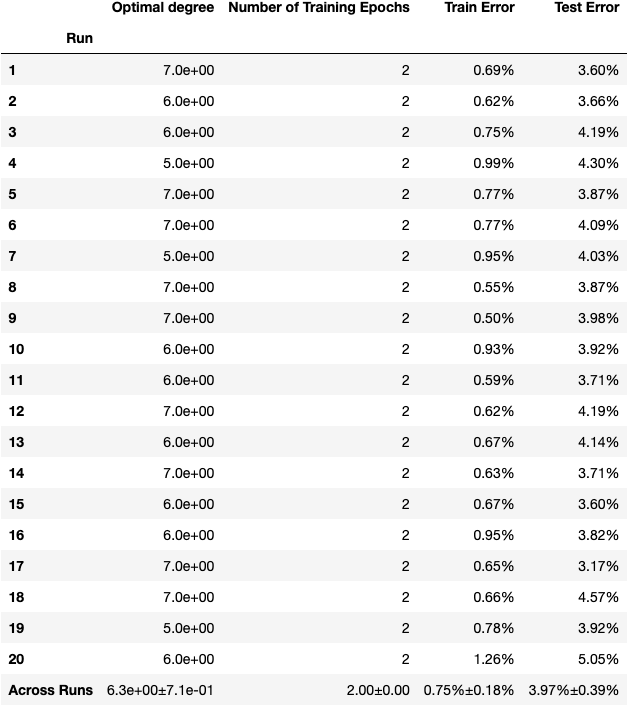
\includegraphics[scale=0.5]{outputs/part1/q6_performance.png}
    \caption{5-fold Cross-Validation for 20 Runs with a Polynomial Kernel (Alternative Training Method)}
    \label{fig:11}
    \end{figure}





\end{itemize}
\newpage
\subsubsection{Discussions}


For these experiments, the number of folds, number of runs, and train/test split were parameters that were arbitrarily chosen, not chosen through cross-validation. Moreover, the kernel parameters were cross-validated to find optimal values, however the range for which cross validation was performed over (i.e. degree 1 to 7 for the polynomial kernel) was chosen relatively arbitrarily. For Gaussian kernels, this was done in a two step process, where a very wide range for sigma was initially used, although this wide range was still chosen arbitrarily. Increasing the number of folds would provide a better estimate of the out of sample performance (i.e. in the limit where we have N folds, each training on $N-1$ points and testing on the single excluded data point). However, this can be quite computationally heavy and a compromise must be drawn. This a similar situation for the number of runs. By increasing the number of runs, we gain a better understanding of average performance, however this is at a computational cost of performing more runs. The train/test split used for these experiments was 80\% training data and 20\% testing data. This follows general rule of thumb for train/test splits. Given a finite data set size, increasing the training percentage can provide inaccurate out of sample performance with the test set. Conversly, a smaller training percentage can poorly represent the model's performance due to limited training examples. Thus a balance must be drawn between the two. The range of hyper-parameters to search for cross validation requires past experience working with kernels and knowledge about the given data set. However these ranges can be quite general (as shown for the Gaussian kernel where we search a space from $1e-05$ to $1e+01$) and we can iteratively narrow our search space.

Comparing the two methodologies for generalising the perceptron to $k$-class classifiers, we can see that the main implementation difference is with the training process, where Algorithm 1 can update an arbitrary number of its weights to be non-zero while Algorithm 2 will update only two weights if the prediction is incorrect. In this sense, Algorithm 1 is like training $k$ independent binary classifiers, where updates are made for each sub-classifier independent of other the prediction of the others. Algorithm 2 introduces dependence between sub-classifiers during the training phase. This is because whether a sub-classifier is selected to be updated depends on if it is the label predicting classifier (i.e. the argmax) or the classifier for the actual label. Otherwise, it is not updated. In some sense, Algorithm 1 is able to pass "correction" signal to all of its classifiers at each step, while Algorithm 2 is constrained in its "speed" of training its classifiers to a maximum of two at a time. Comparing Figure~\ref{fig:2} and Figure~\ref{fig:11}, we can see that Algorithm 1 performs better than Algorithm 2 and this is likely due to this ability of Algorithm 1 to perform corrections for all its classifiers even if they are not the actual label or wrongly predicted label for a training example.

Comparing Figure~\ref{fig:2} and Figure~\ref{fig:9}, we can see that the Gaussian Kernel performs better than the Polynomial Kernel. This is expected because the Gaussian Kernel provides a more expressive (infinite) feature space to model the data compared to a Polynomial kernel.

These experiments were implemented by vectorising and simulating the training behaviour of this online algorithm for faster computation. However, the results exactly mimic the behaviour of the algorithms depicted. The vectorisation starts with initialising a zeros weight matrix $ \textbf{w} = \textbf{0} \in \mathbb{R}^{KxN}$. During the $j^{th}$ step of training, we only update the $j^{th}$ column of weights in $\textbf{w}$. Thus, during prediction for the $j^{th}$ training example, we know that all weights for training examples $\geq j$ will be zero and we will be simulating an online algorithm that only predicts using the $< j$ examples. Moreover during prediction, the operation $\sum_{i'=1}^{i-1} \sum_{j'=1}^{j-1} ( w^{i', j'}_k \cdot  k(\textbf{x}_{j'}, \textbf{x}_j)}$ can be factored as $ \sum_{j'=1}^{j-1} (\sum_{i'=1}^{i-1} w^{i', j'}_k ) \cdot   k(\textbf{x}_{j'}, \textbf{x}_j)}$. Thus, instead of storing a weight matrix of size $\mathbb{R}^{Kx(N \cdot M)}$, for $M$ epochs, we can sum the weights corresponding to the sample training example over multiple epochs and have a weight matrix of constant size $\mathbb{R}^{KxN}$. The kernel evaluations were also precomputed to simulate the online model and speed up computation. Precomputing the gram matrix for a kernel helps vectorise the operation. Thus during the simulated online model, the gram matrix is simply indexed at the appropriate training example to perform the weight updates. Additionally, across different hyper-parameters for a given kernels, a "pre-gram matrix" is pre-computed and used across the different hyper-parameters of a kernel. For example with a polynomial kernel, the gram matrix of inner products is computed as a "pre-gram matrix". Then for each polynomial experiment, the elements of the matrix is simply raised to the $d^{th}$ degree. This also significantly improves the speed of the experiments because a single "pre-gram matrix" can be shared across experiments during a hyper-parameter search. Although the perceptron training algorithm is sequential in nature (i.e. the new weight update depends on the weight updates of the previous step), each hyper-parameter and each run is independent. This invites the opportunity to run these in parallel, performing weight updates for multiple runs in parallel. However we ran into issues of memory constraints when trying to run this on our machine with the given data set, so our implementation did not take advantage of this.


\newpage
\section{PART II}
\subsection{Semi-supervised Learning via Laplacian Interpolation}

Experimental report for the laplacian interpolation approach:
\\
    \begin{figure}[h]
    \centering
    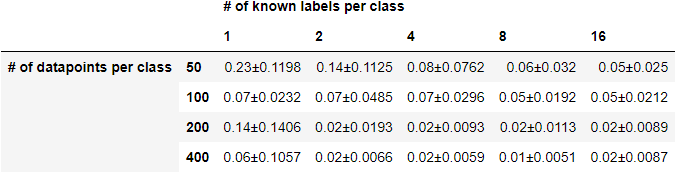
\includegraphics[scale=0.5]{outputs/part2/laplacian_interpolation_report.png}
    \caption{}
    \label{fig:12}
    \end{figure}

\\

And for the laplacian kernel method:
    \begin{figure}[h]
    \centering
    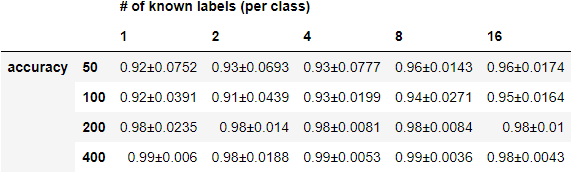
\includegraphics[scale=0.5]{outputs/part2/laplacian_kernel_interpolation_report.png}
    \caption{}
    \label{fig:13}
    \end{figure}

\subsubsection{Discussions}
Both models exhibit high accuracy in all low-data settings. We see here that the vast majority of datapoints are connected only to points
of the same labelling, and that the graph is highly separated into 2 clusters.
Hence with minimal training information, both methods are able to predict with a
high degree of accuracy. For the laplacian seminorm interpolation method, this may be observed 
as its solution in the objective-minimisation form essentially describes a graph cut of minimal size, respecting
the true labels. We should note that in both of our models, the only pints that will be classified incorrectly with a 
reasonably high probability are these teal points in the diagram above.\\

b) Increasing the number of labelled datapoints generally increases the accuracy in both models.\\

c) Increasing the total number of datapoints generally decreases the error variance in the seminorm interpolation
model, but has a limited impact on the kernel interpolation model. \\

d) The laplacian kernel method outperforms the vanilla inerpolation approach considerably, in accuracy, and less so
for variance. \\


The main reason for the success of this algorithm is the high degree of
 cluster separation observed in the dataset.
\\

For illustration, here is a diagram representing the graph adjacency matrix,
 with colours showing the labelling of an edge. Here blue edges are where both 
labels are -1, teal when both are different, and yellow when both are +1.\\


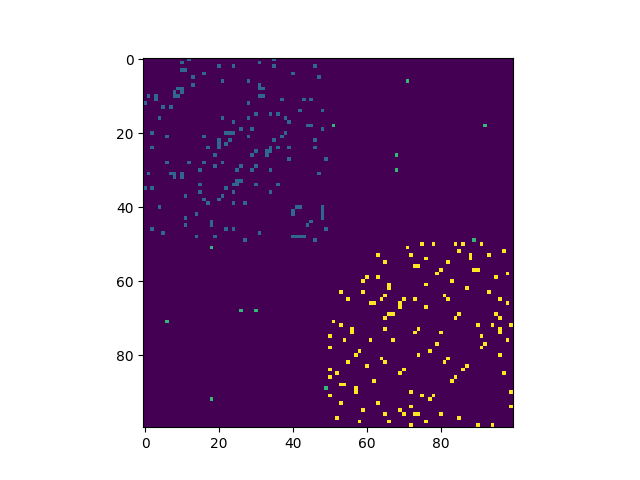
\includegraphics{outputs/part2/graph_label_diagram.png}#

We see through this that the vast majority of datapoints are connected only to points
of the same labelling, and that the graph is highly separated  into 2 clusters.
Hence with minimal training information, both methods are able to predict with a
 high degree of accuracy.\\

Note that error variance decreases as a function of the number of known labels, but 
has a much more significant impact for the vanilla interpolation method.


We see that the kernel approach consistently outperforms the simple laplacian
 interpolation method. A reasonable explanation for this is that the laplacian
interpolation approach utilises local information to 'diffuse' labels through the graph. 
This means that only datapoints close to labelled data receive information from the 
labels themselves, and accuracy is likely reduced for datapoints far from the labels.
In contrast, the kernel interpolation method takes global information from all the 
labelled datapoints and weights them according to their proximity and connectedness 
to eachother to predict labels.
\newpage



\section{PART III}
\subsection{Questions}
\begin{itemize}
    \item[a.] Sample complexity plots for the four algorithms: perceptron, winnow, least squares, and 1-nearest neighbours.


    \begin{figure}[h]
    \centering
    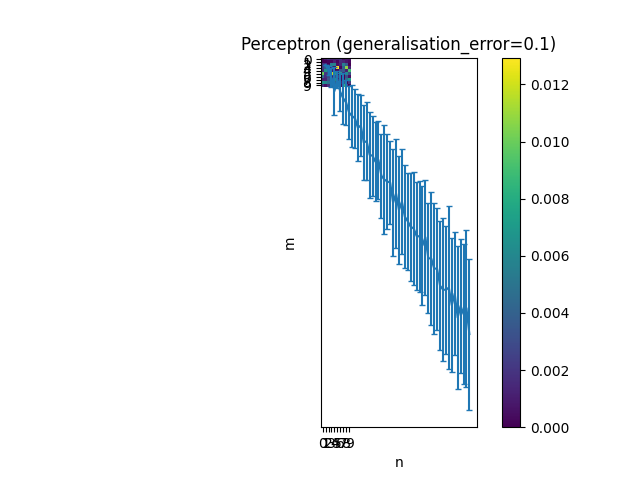
\includegraphics[scale=0.6]{outputs/part3/q1a_perceptron_sample_complexity.png}
    \caption{Perceptron Sample Complexity}
    \label{fig:14}
    \end{figure}


    \begin{figure}[h]
    \centering
    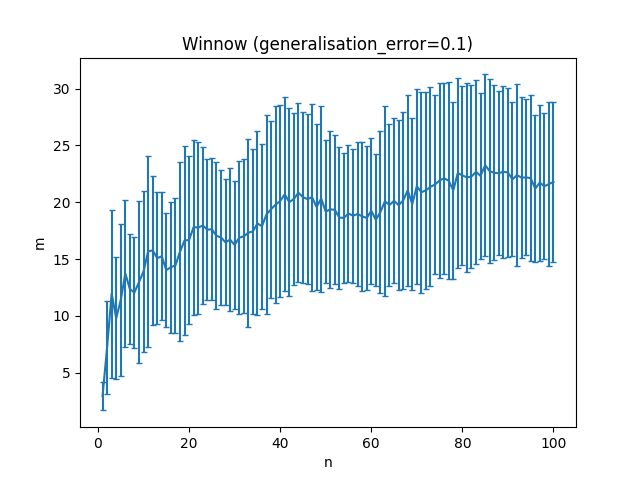
\includegraphics[scale=0.6]{outputs/part3/q1a_winnow_sample_complexity.png}
    \caption{Winnow Sample Complexity}
    \label{fig:15}
    \end{figure}
\newpage
`

    \begin{figure}[h]
    \centering
    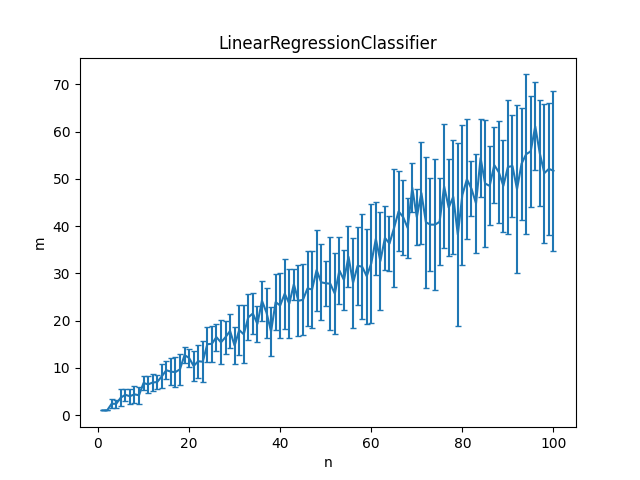
\includegraphics[scale=0.6]{outputs/part3/q1a_lin_reg_sample_complexity.png}
    \caption{Least Squares Sample Complexity}
    \label{fig:16}
    \end{figure}


    \begin{figure}[h]
    \centering
    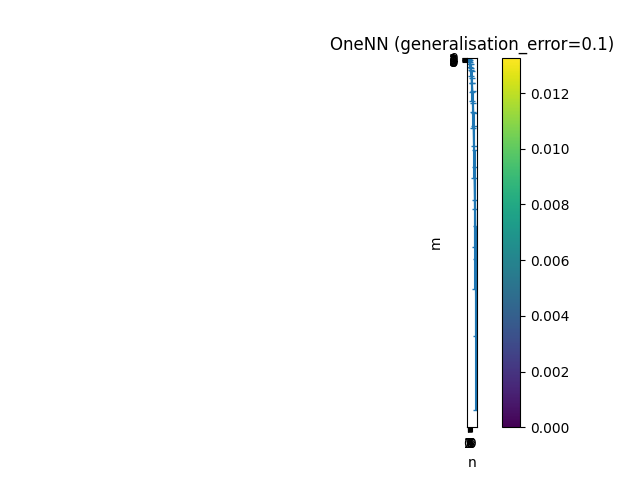
\includegraphics[scale=0.6]{outputs/part3/q1a_one_nn_sample_complexity.png}
    \caption{1-Nearest Neighbours Sample Complexity}
    \label{fig:17}
    \end{figure}


\newpage

    \item[b.] The following algorithm was used to estimate sample complexity:

    \begin{algorithm}
    \caption{Sample Complexity Estimation Algorithm}\label{alg:cap}
    \begin{algorithmic}
    \For{$n\in\{1, 2, ..., N\}$}: \Comment Number of dimensions
        \State $\mathcal{M}_n \gets []$ \Comment Store $m$ values for each trial
        \For {$t\in\{1, 2, ..., T\}$} \Comment Number of trials
            \State $m \gets  0$ \Comment Number of training points
            \State $\mathcal{D}_{train} \gets  \{\}$ \Comment Training set
            \State $\mathcal{D}_{test} \gets  \{(x^1_{test}, y^1_{test}), ..., (x^{M'}_{test}, y^{M'}_{test})\}$ \Comment Fixed test set of size $M'$
            \State $error \gets  1 \Comment initial test set error
            \While{$error > 0.1$}
                \State $m \gets  m+1$
                \State $\mathcal{D}_{train} \gets  \mathcal{D}_{train} \cup \{(x^m_{train}, y^m_{train})\}$ \Comment Add a new training point
                \State $error \gets model.train({D}_{train}).test({D}_{test})$ \Comment Train model and compute error
            \EndWhile
            \State $\mathcal{M}_n \gets \mathcal{M}_n + [m]$
        \EndFor
    \end{algorithmic}
    \end{algorithm}
    For each $\mathcal{M}_n$ the mean and standard deviation were calculated to produce the plots for each model.
    Choosing different values for the number of trials $T$ and the test set size $M'$, is a tradeoff between limited computation resources and accuracy of our approximation. With larger number of trials, we improve our approximation, however this requires more computational resources. A larger test set size $M'$ provides a better approximation of $\{-1 ,1\}^n$ and therefore a better approximation of the generalisation error. Moreover, choosing $N$ puts a finite horizon on the number of points available for estimating the sample complexity function. For some algorithms such as one-nearest neighbours, we see that the number of training samples grows exponentially with $n$. Thus to have a plot up to 100 dimensions like with least squares, would require a lot more computational resources. As such, we limited our evaluation for one-NN to 20 dimensions. However, this can introduce biases in our estimation of the sample complexity. It is possible that our chosen finite horizon is inadequate for capturing the dynamics as $n \rightarrow \infty$. For example, a sample complexity that is actually exponential could seem linear if we do not choose an $N$ that is large enough to reveal this trend.

\newpage
    \item[c.] To estimate how $m$ grows as a function of $n$ as $n \rightarrow \infty$ for each of the four algorithms, we first visualise lines of best fit of the sample complexities for different function classes (i.e. polynomial, exponential, logarithm):


    \begin{figure}[h]
    \centering
    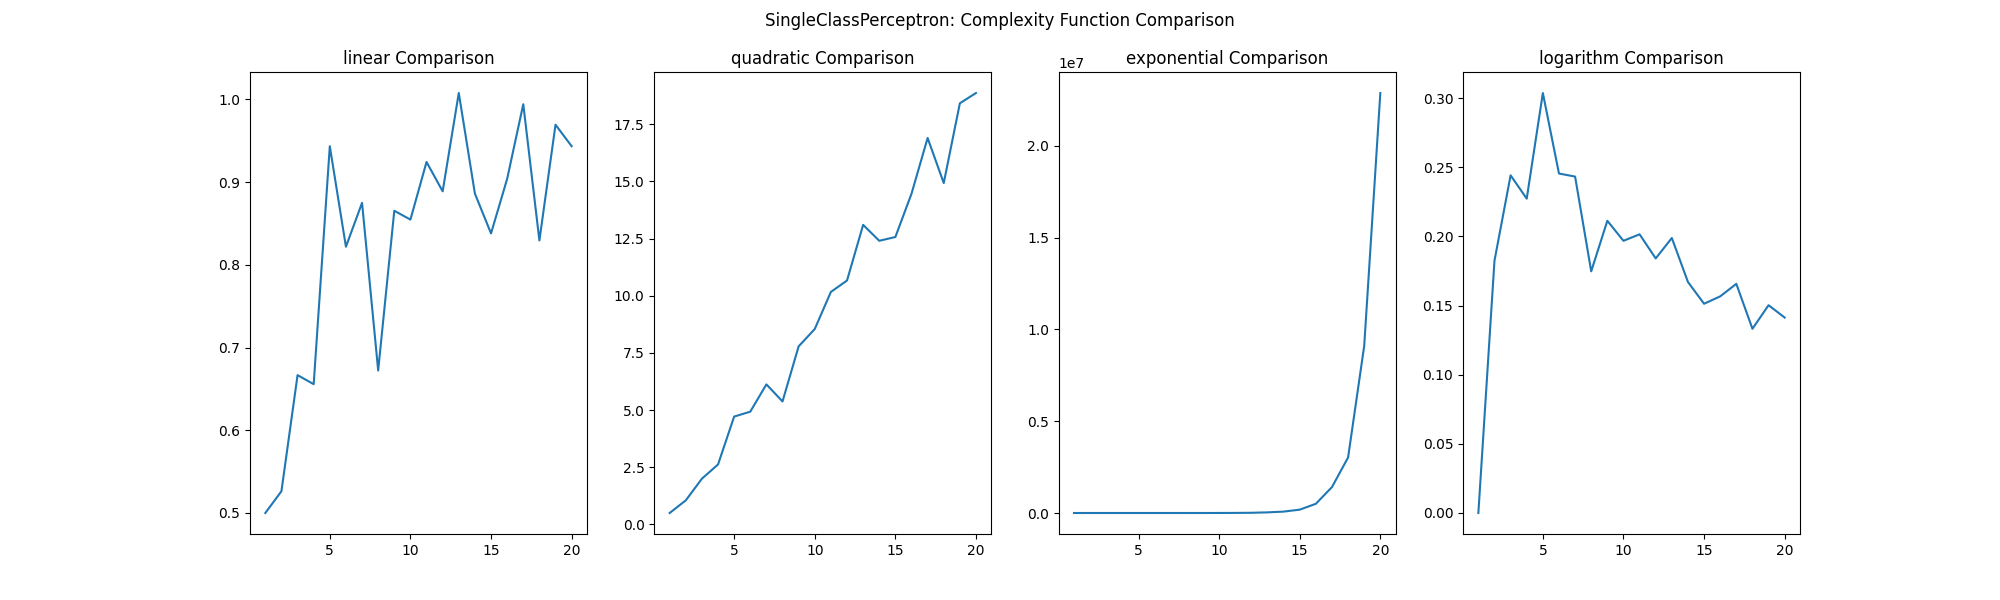
\includegraphics[scale=0.35]{outputs/part3/q1a_perceptron_complexity_function_comparison.png}
    \caption{Perceptron Sample Complexity vs Function Classes}
    \label{fig:18}
    \end{figure}

    \begin{figure}[h]
    \centering
    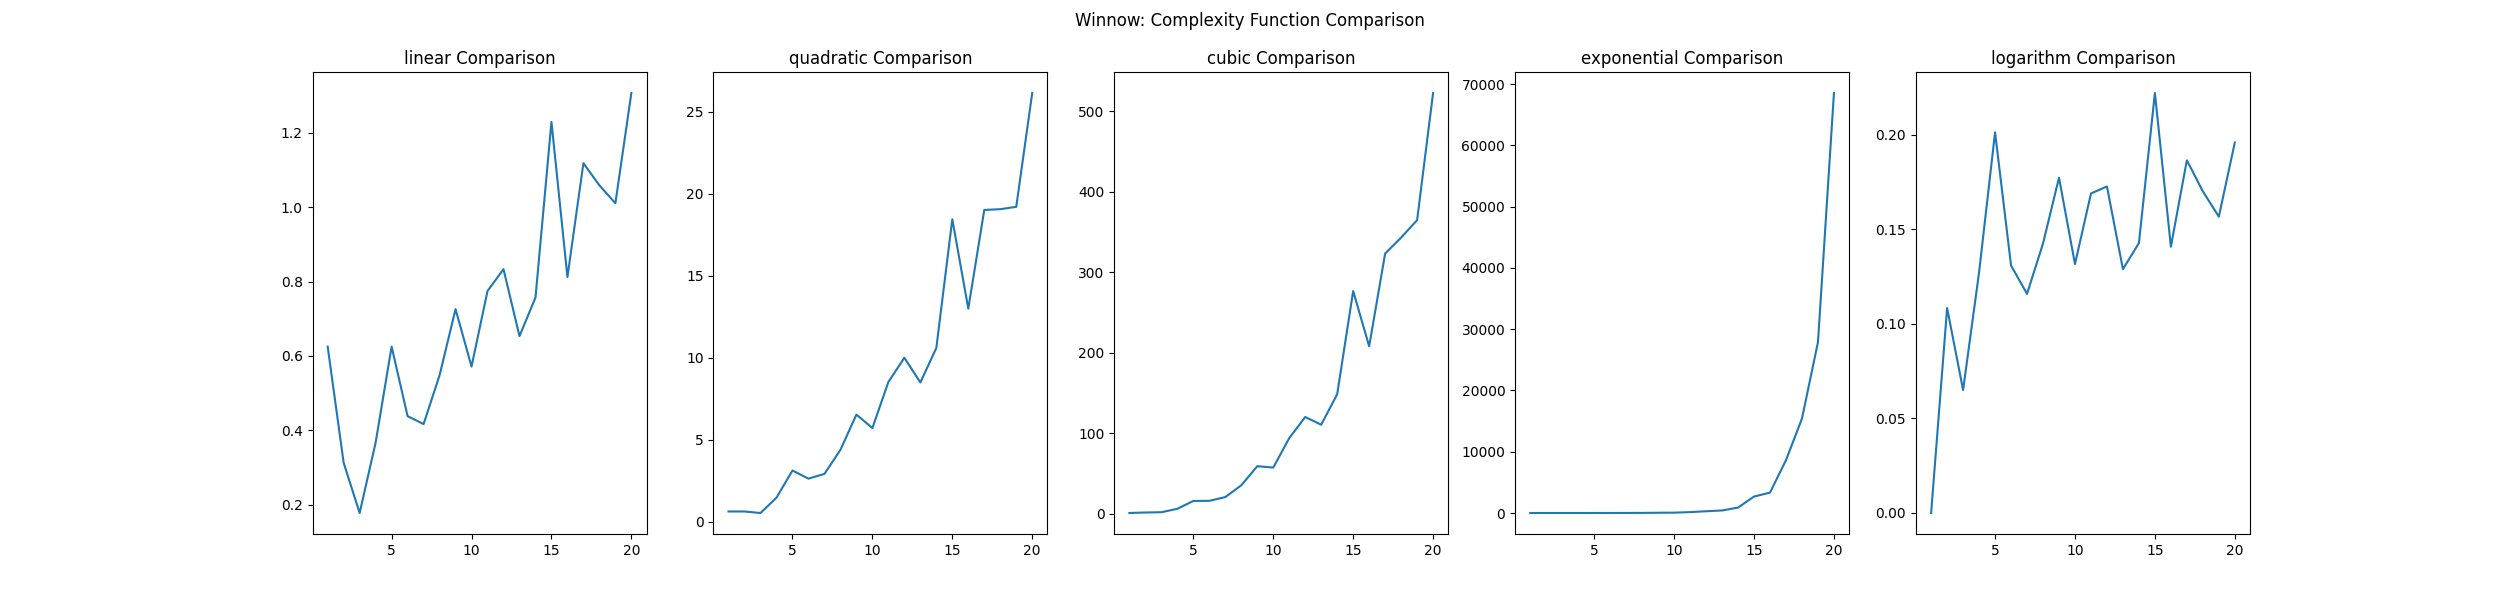
\includegraphics[scale=0.35]{outputs/part3/q1a_winnow_complexity_function_comparison.png}
    \caption{Winnow Sample Complexity vs Function Classes}
    \label{fig:19}
    \end{figure}
\newpage
    \begin{figure}[h]
    \centering
    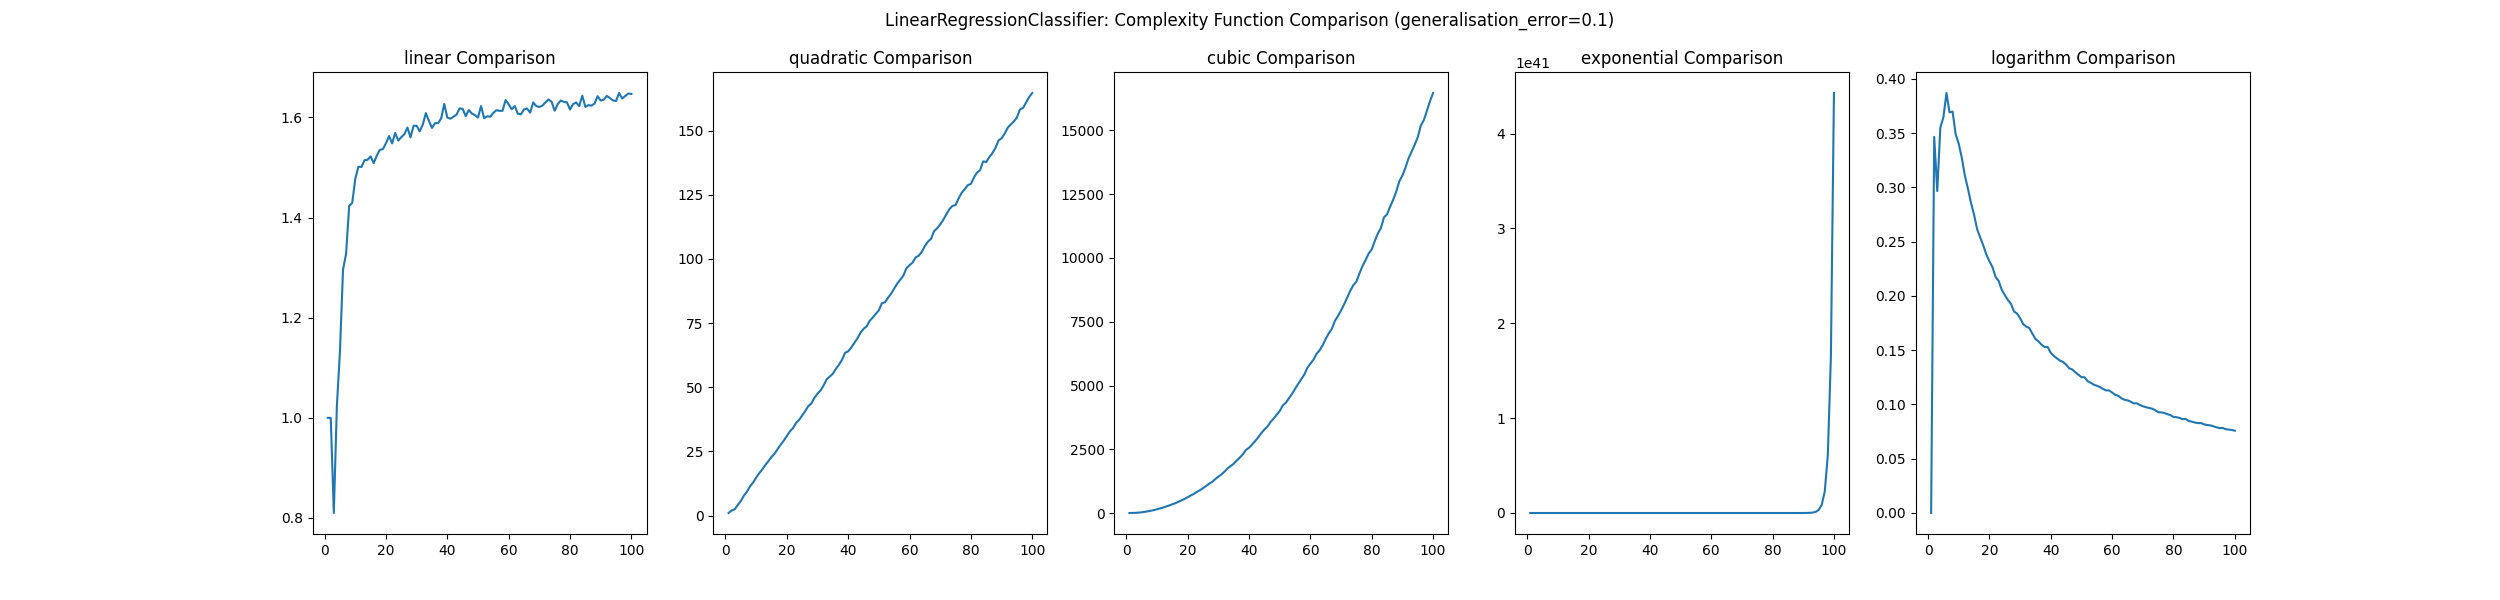
\includegraphics[scale=0.35]{outputs/part3/q1a_lin_reg_complexity_function_comparison.png}
    \caption{Least Squares Sample Complexity vs Function Classes}
    \label{fig:21}
    \end{figure}

    \begin{figure}[h]
    \centering
    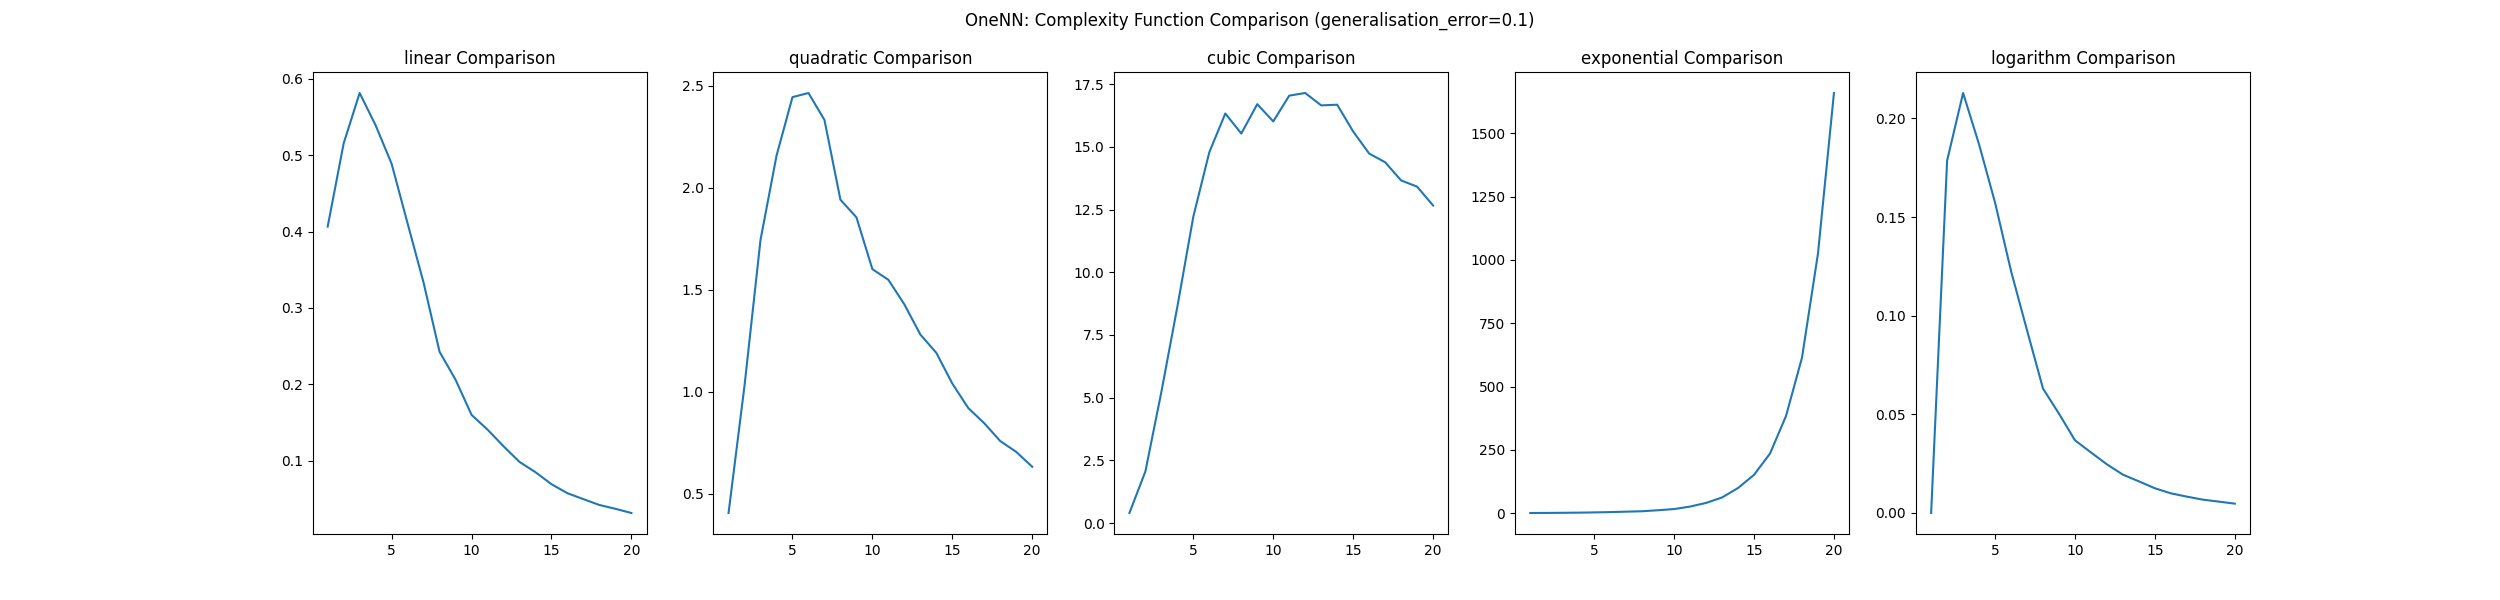
\includegraphics[scale=0.35]{outputs/part3/q1a_one_nn_complexity_function_comparison.png}
    \caption{1-Nearest Neighbours Sample Complexity vs Function Classes}
    \label{fig:22}
    \end{figure}

    From these plots we can see that the perceptron sample complexity grows linearly ($m = \Theta(n)$), the Winnow sample complexity grows logarithmically ($m = \Theta(\log(n))$), the least squares sample complexity grows linearly ($m = \Theta(n)$), and the 1-nearest neighbours sample complexity grows exponentially ($m = \Theta(e^{n})$). These estimates can be qualitatively observed by attempting to fit different function curves to the experimental results and choosing the function with the best qualitative fit. This shows that winnow is a much more robust algorithm in high dimensions due to its logarithmic scaling of the number of training points with respect to the dimensionality to achieve the same error rate. On the other hand, one-nearest neighbours scales exponentially, suggesting that it is impractical to use in high dimensional data. This can be attributed to the curse of dimensionality. Both the perceptron and least squares scale linearly, thus performing worse than winnow but better than the one-NN algorithm.

\newpage

    \item[d.]\\
    We note that since for any $X_{t}$ , $y_{t} = X_{1,t}$ , we have the following
     expression representing the linear separability of our dataset:\\
    \[(v \cdot x_{t})y_{t} \ge 1\]\\
    Where $v = (1,0, \dots, 0)^{T}$. Note that $\|v\| =1$.\\
    Hence, in our online mistake bound for the perceptron, we have that $\gamma =1$.
    Further note that $\forall t$, $x_{t} \in {-1,1}^{n} \implies \|x_{t}\|^{2}
    = n$. This gives us that $R = max_{t} \|x_{t}\| = \sqrt{n}$.
    Hence our mistake bound for the perceptron algorithm is given by:\\
    
    \[M \le n \].\\

    Using the theorem on page 60 of the online learning notes, we arrive at:\\

    \[Prob(\mathcal{A_{S}}(x ^{\prime}) \ne y^{\prime} ) \le \frac{n}{m}\]\\

\newpage

     \item[e.]\\
     From our experimental observations we may expect the sample complexity of 1-NN
     to be lower bounded by some exponential function. We formalise this in the
     following proposition:\\

    \textbf{Proposition:}\\

    Following the data-generating distribution described above, we have that our sample complexity given by:\\

    $m(n) = \Omega (n)$ \\
    \textbf{Proof:}\\

    Suppose we sample a training set $S = \{(x_{1},y_{1}), \dots, (x_{n},y_{n})\} $ uniformly from the set $\{-1,1\}^{n}$, with associated labels
    defined by the rule $y | x = x_{1}$, and use this training set for inference on an
     arbitrary test point $(x,x_{1})$, sampled uniformly from the same set.
    \\
    We note the following observation:\\

    \textbf{Obs:}\\
    if $x \in S$, then $\mathcal{A}_{S}(x)) = y$, where y is the true label for x. \\

    To justify this, observe that our dataset represents a realiseable learning problem,
    and as such, if $(x,y), (x \prime,y \prime)$ are datapoints sampled from our distribution,
    $x = x \prime \implies y = y \prime $. Trivially, x is the 1-nearest neighbour to itself,
    so the algorithm makes a correct prediction for any datapoint present in our training set.\\

    Hence, $\mathcal{A}_{S}$ makes an error on x $\implies x \notin S$.
    
    Hence, the set of all training sets that make an error on x is contained in the set of all
    training sets not containing x. \\

    Hence, for a given x, $P_{S}(\mathcal{A}_{S}(x) \ne y) \le P_{S}(x \notin S)$.\\

    Since S is a collection of points sampled iid from our data generating distribution, \\
    $P_{S}(x \notin S) = \prod_{i=1}^{m}P(x_{i} \ne x) = \prod_{i}(1 - P(x_{i} = x)) = (1 - 2^{-n})^{m}$\\

    We note that our choice of x was arbitrary, and since we sampled x uniformly, we arrive at the 
    following generalisation error bound:\\

    $\mathbb{E}_{S \sim \mathcal{D}^{m}, x \sim \mathcal{D}}[\mathcal{L}_{S}(x)] \le (1 - 2^{-n})^{m} $\\
    Using the identity $1-x \le e^{-x}$ provided frequently in the notes, we simplify this bound to give:
    \\
    \\

    $\mathbb{E}_{S \sim \mathcal{D}^{m}, x \sim \mathcal{D}}[\mathcal{L}_{S}(x)] \le exp(-2^{n}m)$
    \\
    Suppose we seek m such that our generalisation error is less than some fixed $\epsilon$. \\
    \\
    Hence we require $\mathbb{E}_{S \sim \mathcal{D}^{m}, x \sim \mathcal{D}}[\mathcal{L}_{S}(x)] \le exp(-2^{n}m) \le \epsilon$\\
    \\
    $\implies -m2^{-n} \le log(\epsilon)$\\

    Hence, $m \ge -log(\epsilon)2^{n} = log(\frac{1}{\epsilon}) 2^{n}$\\

    $\implies m = \Omega(2^{n})$\\
    $\square$
\end{itemize}
\end{document}
